\section{Implementing the editor calculus}

The implementation of the editor calculus requires

\begin{itemize}
\item implementing the semantics of the calculus and allowing for an
  appropriate visualization of editing
\item implementing a type checker based on the type system
\end{itemize}

but perhaps surprisingly, it involves finding a way to script editor
calculus expressions. In this section we outline this.

\subsection{Implementing the editor calculus semantics}

We model the formation rules of the editor calculus by a collection of
algebraic datatypes. As an example, expressions are given by the
datatype

\begin{lstlisting}[language=elm,%
                   label={aep-without-holes-definition},%
                   gobble=4,%
                   caption={Formation rules (\ref{aep-formation-rules}) modeled in Elm},%
                   ]
    type Aep
        = Eval
        | Sub Aam
        | Child Ast.Child
        | Parent
\end{lstlisting}

The rest of the formation rules are defined similarly.

\subsection{Abstract syntax trees}

We are interested in visualizing the AST to make the editor intuitive
for a user.  We are not necessarily interested in finding the ``best''
visualization, nor in implementing a vast number of different
representations.

A simple representation would be to represent the AST in a textual form,
as seen in figure \ref{fig:ast-in-text-form}.

\begin{figure}[H]
    \Large
    \begin{equation*}
      \cursor{(\app{\breakpoint{(\lambda{x}{(\app{x}{x})})}}
      {(\lambda{x}{(\app{x}{x})})})}
    \end{equation*}
    \caption{An AST visualized in textual form.}
    \label{fig:ast-in-text-form}
\end{figure}

The notation used for this representation follows that of Godiksen
et al.~\pepm. It is straightforward but can also be
difficult to reason about, especially as the AST grows large.

We also implement another representatio, namely as a tree as seen in
figure \ref{fig:ast_visual_tree}.

Switching between the two visualizations is immediate in the user interface.

\begin{figure*}
  \center
  \noindent\begin{minipage}{.45\textwidth}
    \center
    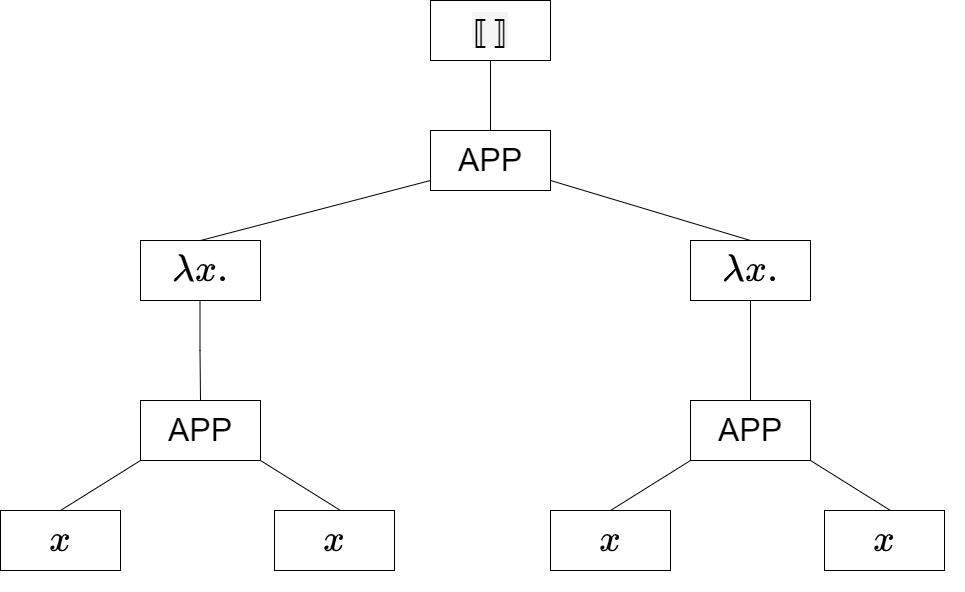
\includegraphics[width=\textwidth]{assets/ast_root_cursor.png}
  \end{minipage}\hfill
  \begin{minipage}{.45\textwidth}
    \center
    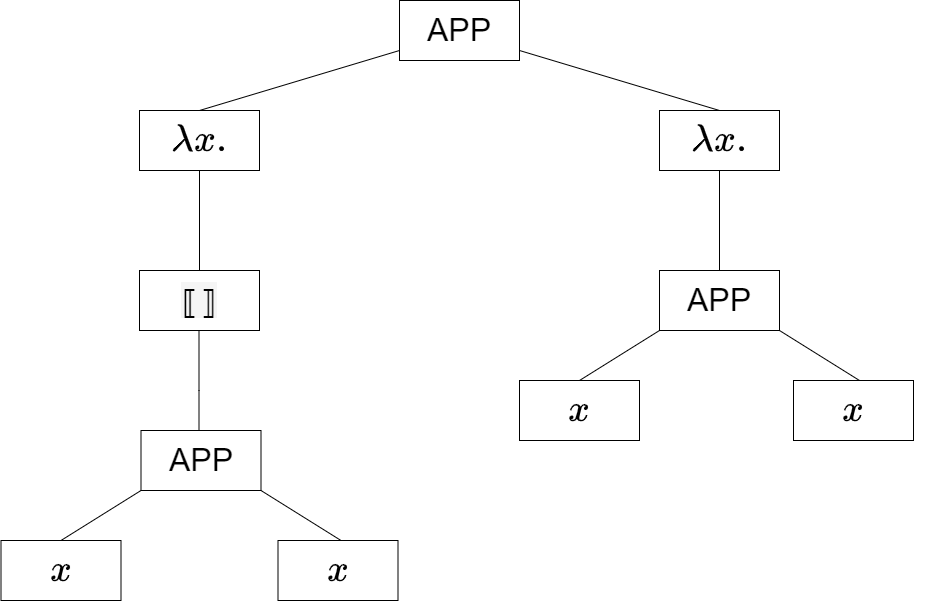
\includegraphics[width=\textwidth]{assets/ast_subtree_cursor.png}
  \end{minipage}\hfill
  \caption{An AST before and after cursor movement visualized in tree form}
  \label{fig:ast_visual_tree}
\end{figure*}

\subsection{Implementing a type checker}

We type check with respect to a
configuration. We say that a configuration is well-typed iff; the AST is both
well-formed and well-typed in the empty AST context and the editor expression
is both well-formed and well-typed for the path to the cursor in the AST and
the editor context containing all valid paths in the AST \pepm. I.e. equation
(\ref{eq:welltypedconf}) where $\emptyset$ is the empty AST context, $p$ is the
path from the root to the cursor in $a$, and $\ctx{e}$ is the editor context
containing some pair for each valid path in $a$.

\begin{equation}\label{eq:welltypedconf}
  \TConfiguration
\end{equation}

\subsection{Building editor expressions}
Editor expressions written in a text field would have to be lexed and parsed.
This introduces syntax errors to the editor with regards to editor expressions,
which goes against the spirit of the editor. Hence we created an builder to
build editor expressions in a similar manner to ASTs.

To build editor expressions, we need to introduce holes to the editor
expressions. We define a hole term constructor for each type of editor
expression, as seen in figure \ref{fig:editorexpressionswithholes}

\begin{figure}[H]
    \center
    \begin{tabular}{llll}

        \begin{lstlisting}[language=elm,%
                            gobble=8,%
                            mathescape,%
                            ]
             type Aep
                = Eval
                    $\vdots$
                | AepHole
        \end{lstlisting} &

        \begin{lstlisting}[language=elm,%
                            gobble=8,%
                            mathescape,%
                            ]
            type Eed
                = Neg Eed
                     $\vdots$
                | EedHole
        \end{lstlisting} \\

        \begin{lstlisting}[language=elm,%
                            gobble=8,%
                            mathescape,%
                            ]
            type Edt
                = Pre Aep Edt
                    $\vdots$
                | EdtHole
        \end{lstlisting} &

        \begin{lstlisting}[language=elm,%
                            gobble=8,%
                            mathescape,%
                            ]
            type Aam
                = Var Var.Id
                    $\vdots$
                | AamHole
        \end{lstlisting}
    \end{tabular}
    \caption{Editor expression definitions with holes}
    \label{fig:editorexpressionswithholes}
\end{figure}

We are now able to build editor expressions by initializing the editor
expression builder with an \texttt{EdtHole}, and then allow the user to
substitute holes with appropriate expressions. As with ASTs, we have the concept
of atomic editor expressions, which are editor expressions with holes as
children. The user can substitute holes until no holes are left. An editor
expression without any holes is said to be \textit{completed}.

We are only interested in evaluating completed editor expressions. To do this,
we introduce a type variable to each editor expression type. The type variable
is used for recursively defining the type in terms of the type variable, but
also as an argument to each hole constructor, as seen in the following
listing.

\begin{lstlisting}[language=elm,%
                   label="eed-definitions",%
                   gobble=4,%
                   ]
    type Eed a
        = Neg (Eed a)
        | Conjunction (Eed a) (Eed a)
        | Disjunction (Eed a) (Eed a)
        | At (Aam a)
        | Possibly (Aam a)
        | Necessarily (Aam a)
        | EedHole a
\end{lstlisting}

We utilize the \texttt{()} and the \texttt{Never} types to represent
completed and uncompleted editor expressions. If for example \texttt{a} in
\texttt{Edt a} is replaced with \texttt{()}, the editor expression can contain
holes. Conversely, if we replace \texttt{a} with \texttt{Never}, it cannot
contain holes, since we need a \texttt{Never} value to construct a hole. We can
therefore use \texttt{Edt ()} to represent uncompleted editor expressions, and
\texttt{Edt Never} to represent completed editor expressions. We have created a
type alias for completed and uncompleted editor expressions of every type.

This approach creates strong guarantees by making impossible states impossible.
The \texttt{toCompleted} function cannot take an \texttt{uncompleted} editor
expression, return a \texttt{completed} editor expression and still have bugs,
since we have constrained the types to create type level guarantees.

\subsection{The user interface}
\label{user-interface}

The user interface allows for two different visualizations of
programs: a textual representation and a tree representation. The
implementation of the textual representation is simple: A conversion
of the AST data structure to HTML with syntax highlighting . The last
image in figure \ref{fig:final_ui} shows this.

The implementation of the tree representation is more involved. Figure
\ref{fig:ast_visual_tree} shows an example of this

The visualization of the editor expression builder is similar to the textual
representation of ASTs. We implemented a function that given an \texttt{Edt}
returns HTML. An example of an
editor expression being built is in the upper left corner of the images in
figure \ref{fig:final_ui}.

\begin{figure*}
  \center
  \noindent\begin{minipage}{\textwidth}
    \center
    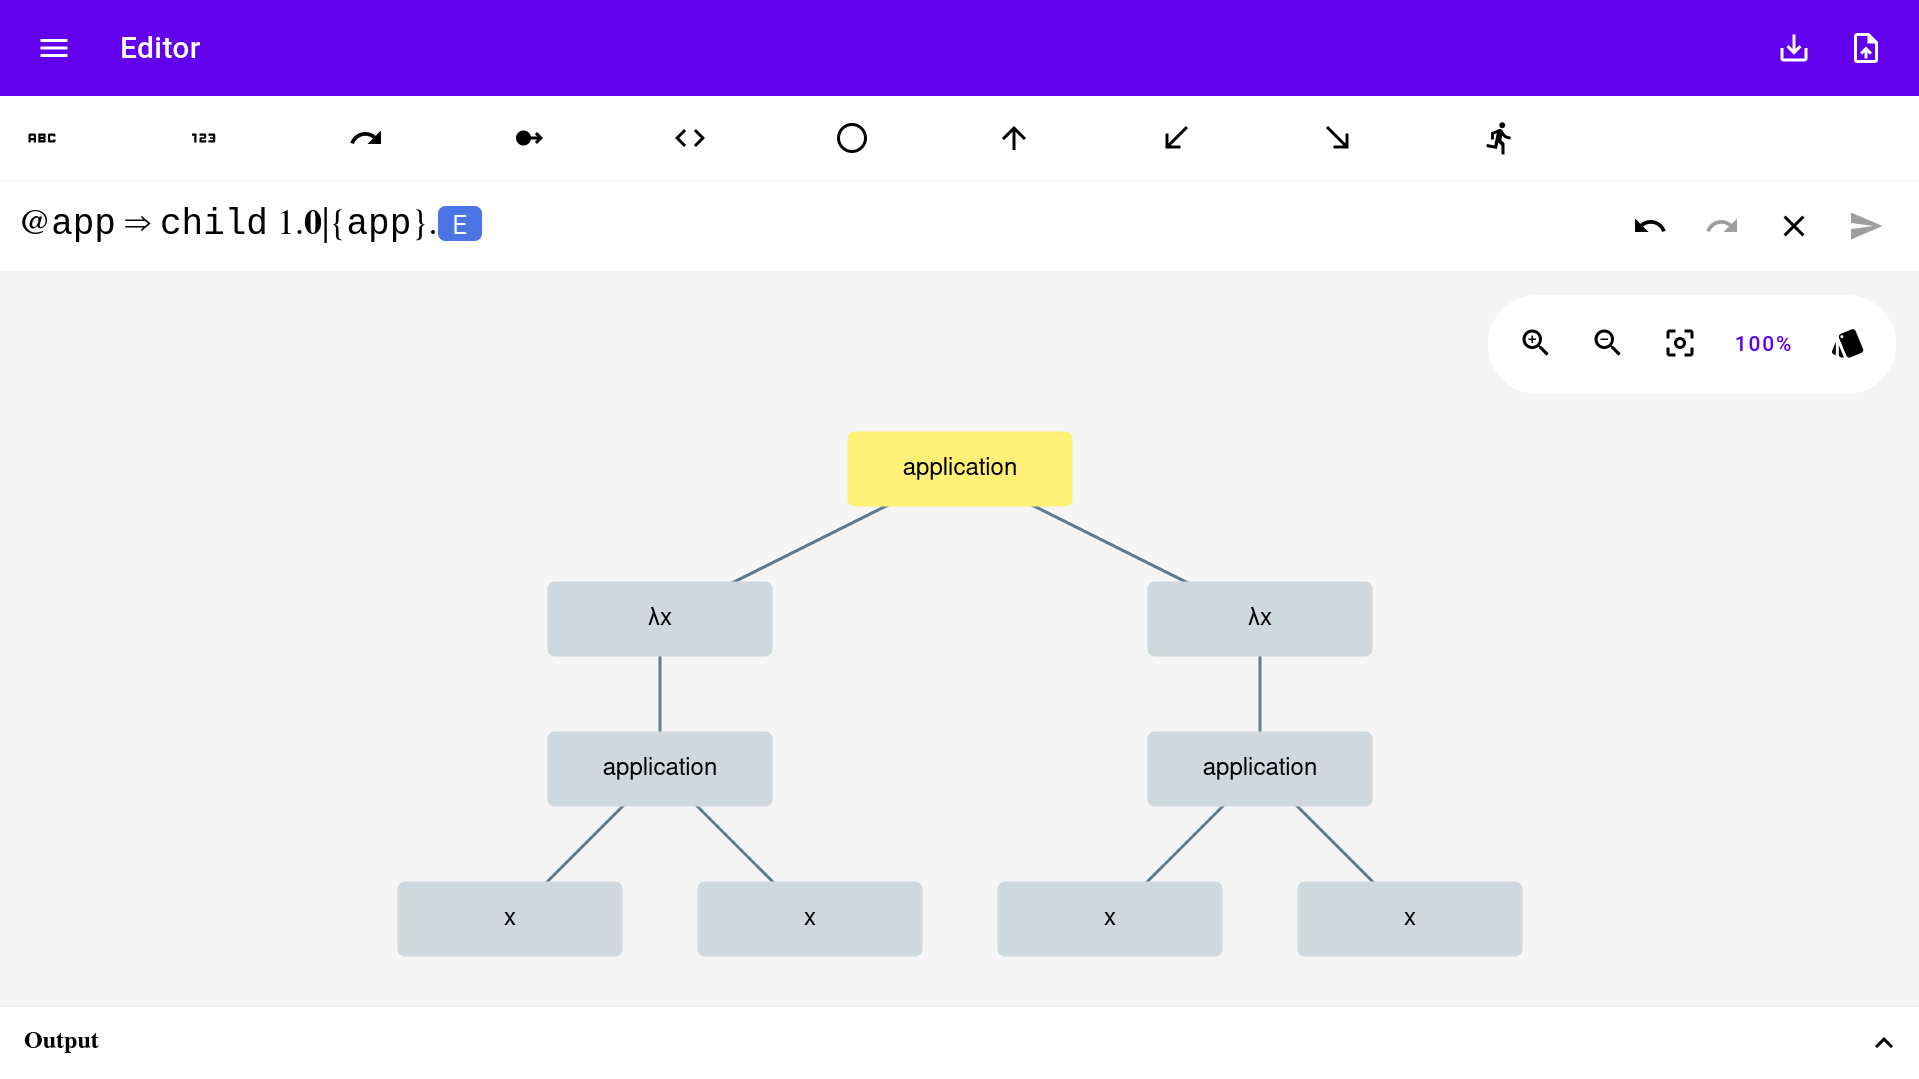
\includegraphics[width=0.7\textwidth]{assets/final_ui1.png}
  \end{minipage}\hfill
  \begin{minipage}{\textwidth}
    \center
    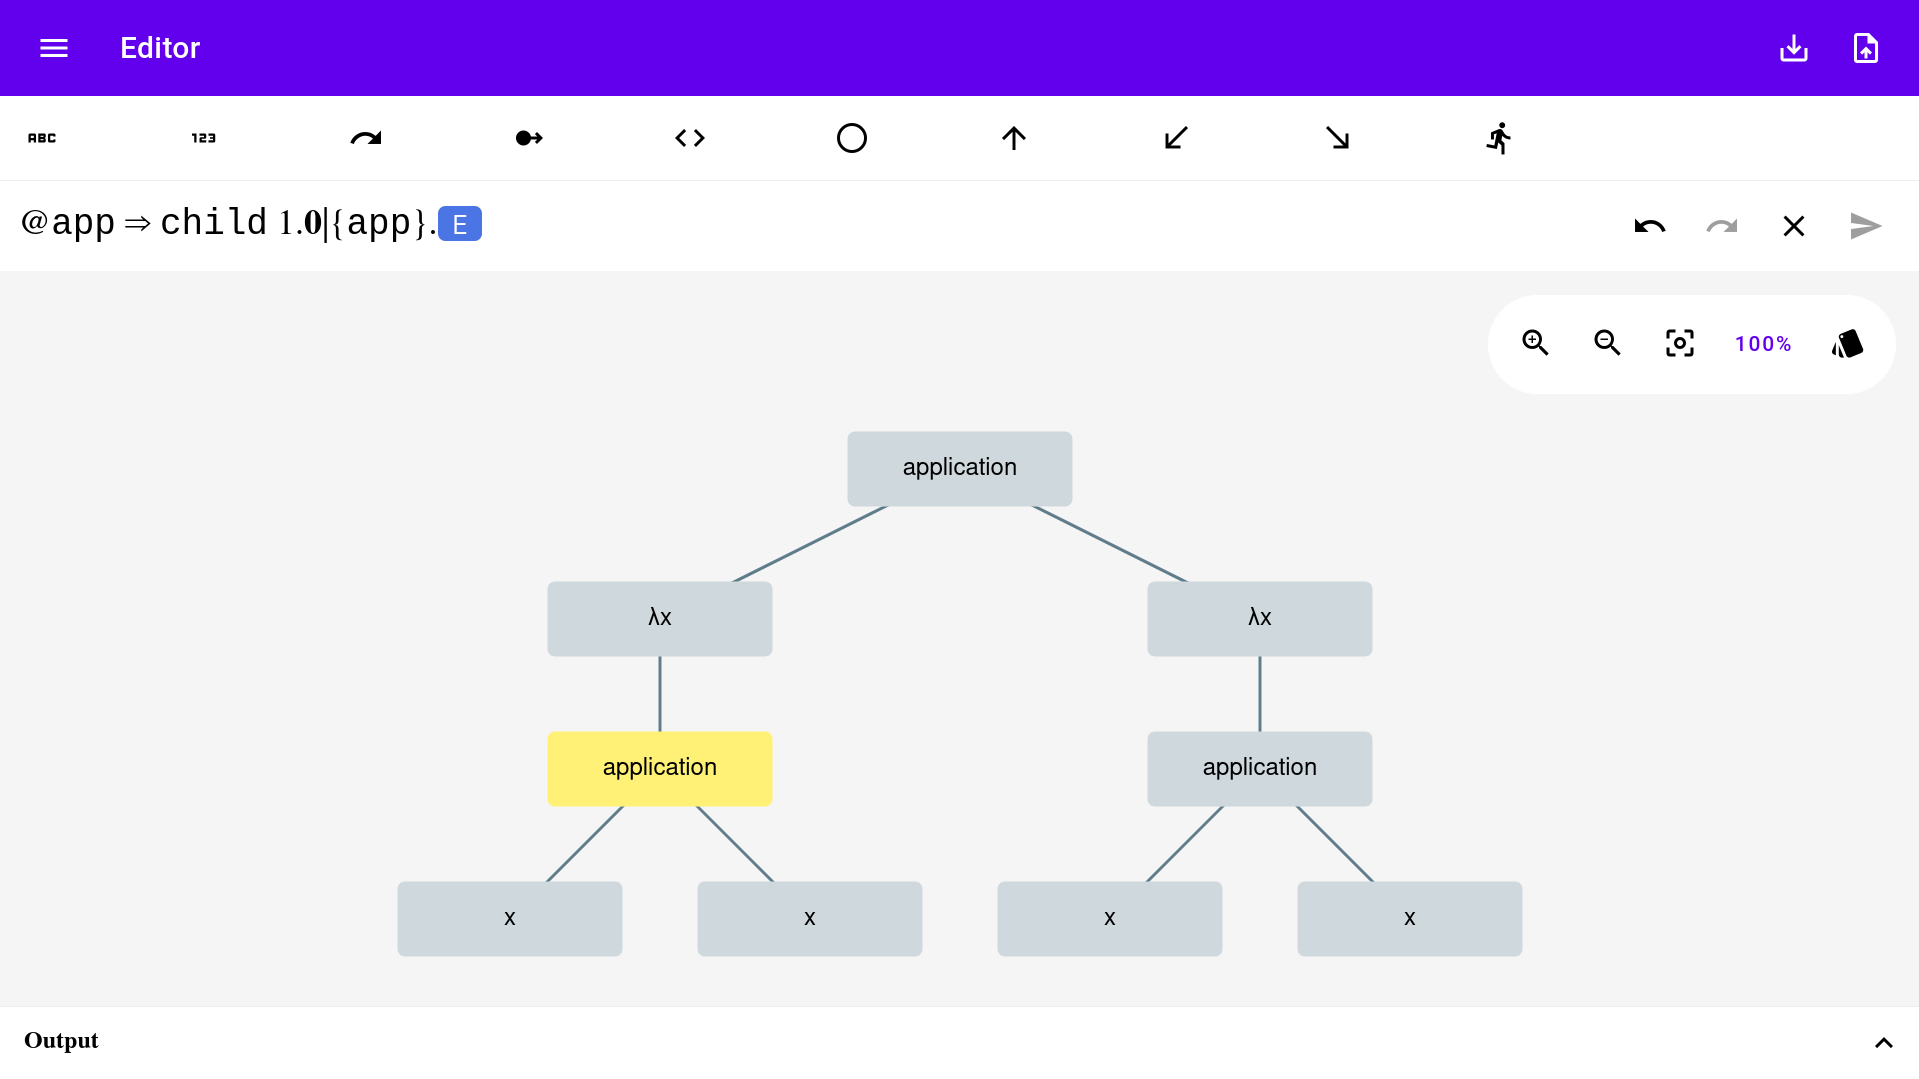
\includegraphics[width=0.7\textwidth]{assets/final_ui2.png}
  \end{minipage}\hfill
  \begin{minipage}{\textwidth}
    \center
    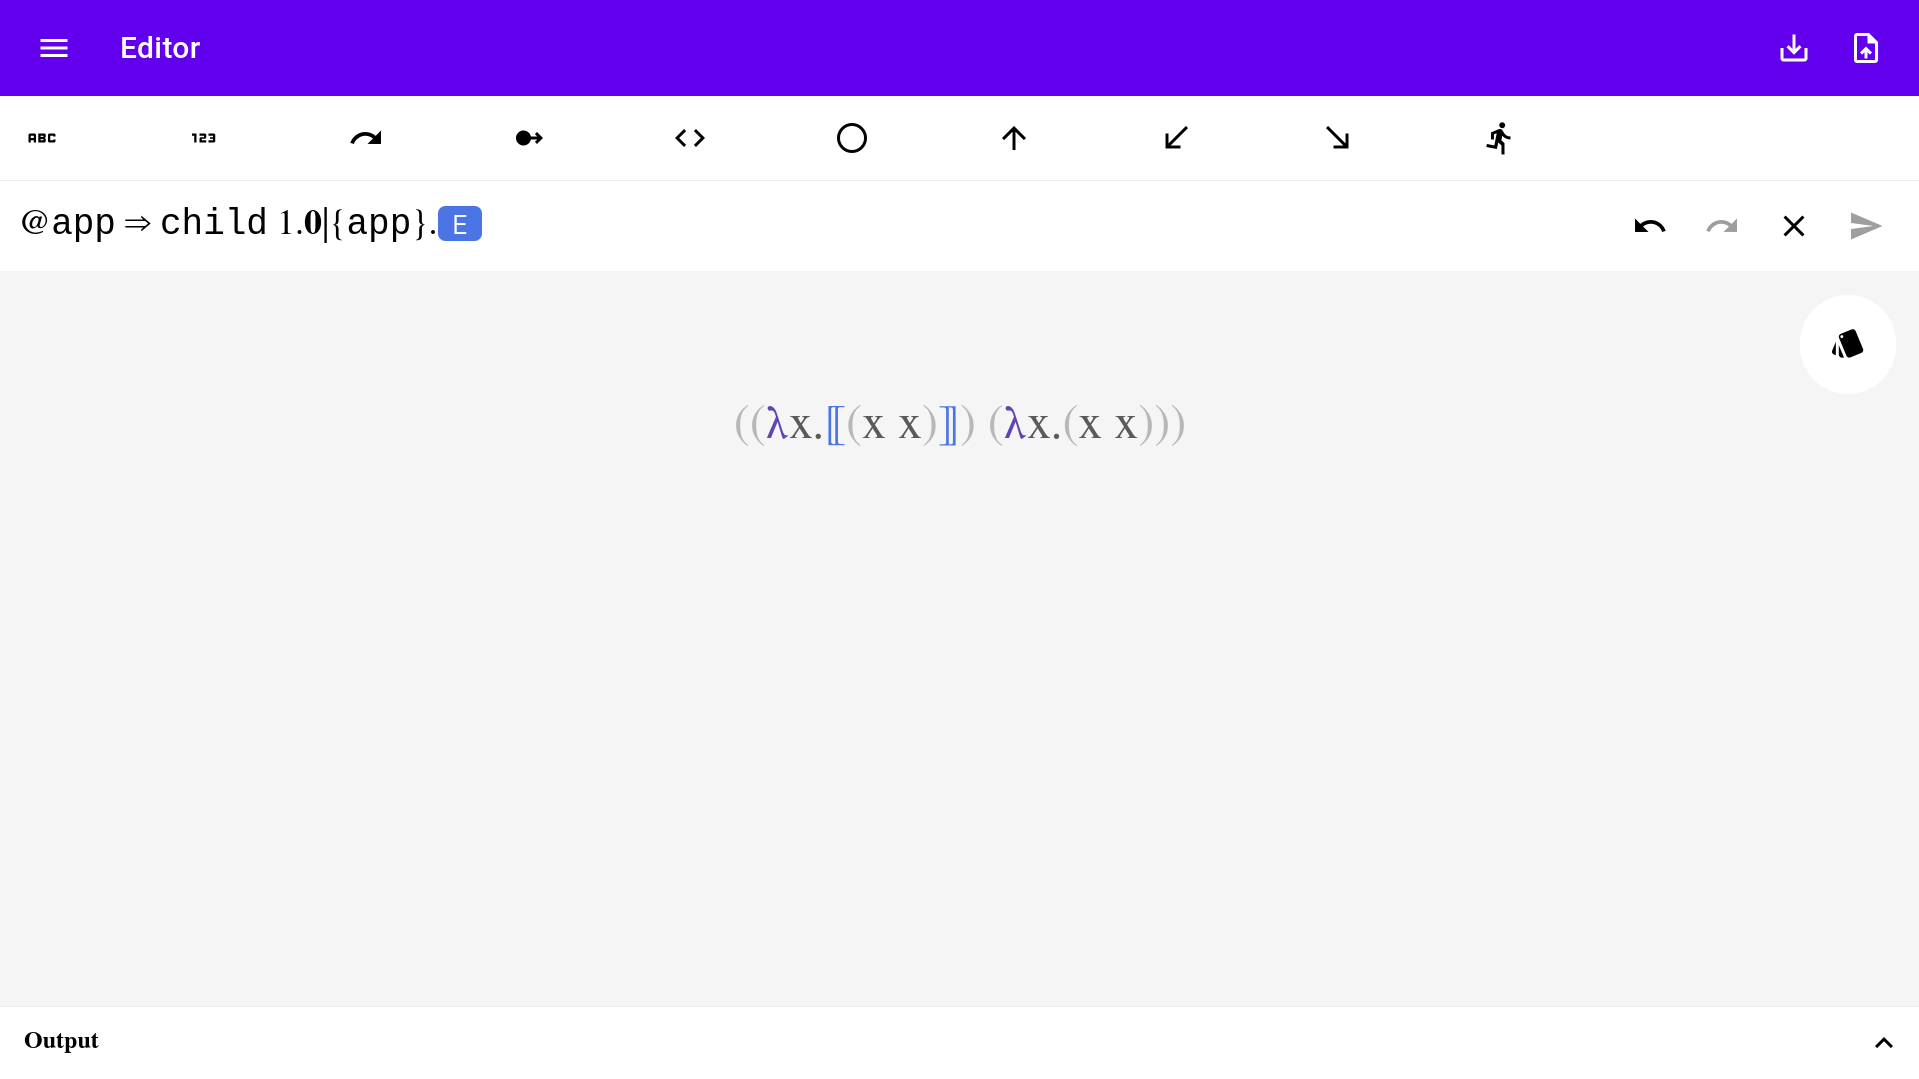
\includegraphics[width=0.7\textwidth]{assets/final_ui3.png}
  \end{minipage}\hfill
  \caption{The figures \ref{fig:ast-in-text-form} and \ref{fig:ast_visual_tree} from section \ref{design} recreated in the final UI}
  \label{fig:final_ui}
\end{figure*}

%%% Local Variables:
%%% mode: latex
%%% TeX-master: "../pepm2023"
%%% End:

\subsection{Conditions}

\begin{figure*}
  \center
  \renewcommand{\arraystretch}{2}
  \begin{tabular}{llllll}
    \scriptsize(AT-VAR)      & $\AtVar$      & \scriptsize(AT-CONST)  & $\AtConst$   & \scriptsize(AT-HOLE)   & $\AtHole$   \\
    \scriptsize(AT-APP)      & $\AtApp$      & \scriptsize(AT-ABS)    & $\AtAbs$     & \scriptsize(AT-BREAK)  & $\AtBreak$  \\
    \scriptsize(POS-TRIVIAL) & $\PosTrivial$ & \scriptsize(POS-ABS)   & $\PosAbs$    & \scriptsize(POS-BREAK) & $\PosBreak$ \\
    \scriptsize(POS-APP-1)   & $\PosAppOne$  & \scriptsize(POS-APP-2) & $\PosAppTwo$ &   \scriptsize(NEC-TRIVIAL) & $\NecTrivial$ \\
    \scriptsize(NEC-APP)     & $\NecApp$     & \scriptsize(NEC-ABS)   & $\NecAbs$    & \scriptsize(NEC-BREAK) & $\NecBreak$
  \end{tabular}
  \caption{Condition reduction rules}
  \label{fig:conditionreductionrules}
\end{figure*}

The checks for the three modalities are implemented in the functions
$\elm{isEquivalent}$, $\elm{possibly}$ and $\elm{necessarily}$, and checks the
current AST under the cursor.

For the $\elm{isEquivalent}$ function the
\hyperref[fig:conditionreductionrules]{(AT-...)} rules are implemented by a
pattern match over the parameters.
The function applies the rules very straightforwardly such that if one of the
clauses holds then it returns $\elm{True}$ and if not then it returns
$\elm{False}$, where the only addition is the usual $\elm{never}$ function
for a node modifier hole. In rule
\hyperref[fig:conditionreductionrules]{(AT-CONST)} it is not clear whether the
constants have to be equal or just some constant in order for $\at(\const c)$ to
hold. We chose that the constants must be equal.
For all three of the functions, we discard unused parameters of the term
constructors, such as variable IDs and type annotations.

The $\elm{possibly}$ function is reduced by first checking whether we have the
trivial case \hyperref[fig:conditionreductionrules]{(POS-TRIVIAL)}. If we do
not, we check whether any of the other rules holds, i.e. if we are at an
application, abstraction or breakpoint, it calls recursively on the children of
the AST node. It deviates from the rules in that it combine the rules
\hyperref[fig:conditionreductionrules]{(POS-APP-1) and (POS-APP-2)} by a logical
or-operator.

The $\elm{necessarily}$ function is implemented in the same manner as
$\elm{possible}$, with the only difference being if it is not the trivial case
and the AST node is an application, then it uses a logical and-operator instead
of a logical or-operator.
